In this chapter we introduce some basic, required background for this thesis. First, we introduce light probes and the mathematical equations that define them. Then, we present the AI architecture that was the basis of our AI model. Finally, the tools and technologies used for this thesis are presented.

\section{Light Probes}
As mentioned previously, the idea of using discrete probes to capture scene lighting data traces back to early GI research. In the paper \parencite{Greger1998} introduced the irradiance volume, a 3D grid of sample points storing the irradiance field to approximate GI in complex scenes. A light probe samples the incident radiance at a point in empty space from all directions. Often just the diffuse component of the radiance is captured, since it most commonly varies smoothly, so it can be compactly represented by projecting the lighting onto a truncated spherical harmonic (SH) basis. Third-order SH is most commonly used, storing 9 coefficients per color channel, abbreviated to L2-SH.

\begin{figure}[h]
	\centering
	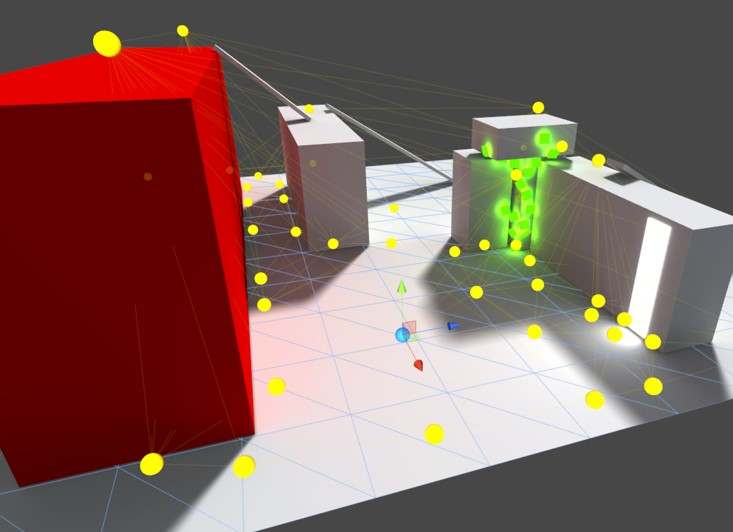
\includegraphics[scale=0.5]{Graphics/light_probes.jpg}
	\caption{A 3D Scene showing a few light probes placed in important locations \parencite{Unity2016}.}
	\label{fig:Light_probes}
\end{figure}


\section{Spherical Harmonics}
Spherical Harmonics (SH), first introduced by Pierre Simon de Laplace, are a method of storing information on a point in space. They are categorized in structures called orders. We are interested in third-order SH, since they represent a good middle ground between storage size, computational cost and accuracy. SH are often described as the Fourier Series of functions on the surface of a sphere, breaking down any pattern of light on a sphere into a set of basis frequencies. The order of SH depicts the amount of data we capture, third-order SH, noted as L2 SH, store the first three bands of data, resulting in 9 coefficients per color channel. Bands represent the individual frequencies; the Zeroth band captures the overall average lighting present in that position in space, the First band captures simple directional gradients, and the Second band captures quadratic variations, e.g. gentle light gradients and their shadows.

\section{PointNet}
\label{sec:background:pointnet}
PointNet \parencite{PointNet2017} is a neural-network architecture designed to work directly on unordered 3D point-clouds; a collection of points without any required grid connectivity. Each point passes through a small MultiLayer Perceptron (MLP), extracting a feature vector that describes its local attributes, e.g. color and normal. After per-point features are computed, PointNet aggregates them into a global descriptor by applying a symmetric operation, usually max-pooling across all points, capturing the strongest signal from the features. Then, the global descriptor is concatenated back to the per-point features, resulting in every point having knowledge about both its characteristics and the broader context. Finally, a per-point MLP refines these combined values into task-specific outputs, commonly classification scores or per-point importance metrics.

Since there is no fixed grid, meaning the points are assumed to be unordered and irregular, traditional CNNs can't be applied directly. Additionally, since PointNet predicts values per-point, it can be used to handle point clouds of any shape and point amount without retraining, limited only by the system's memory. This makes PointNet a fitting candidate to base our model on, with the implementation being the only varying factor.

\begin{figure}[h]
	\centering
	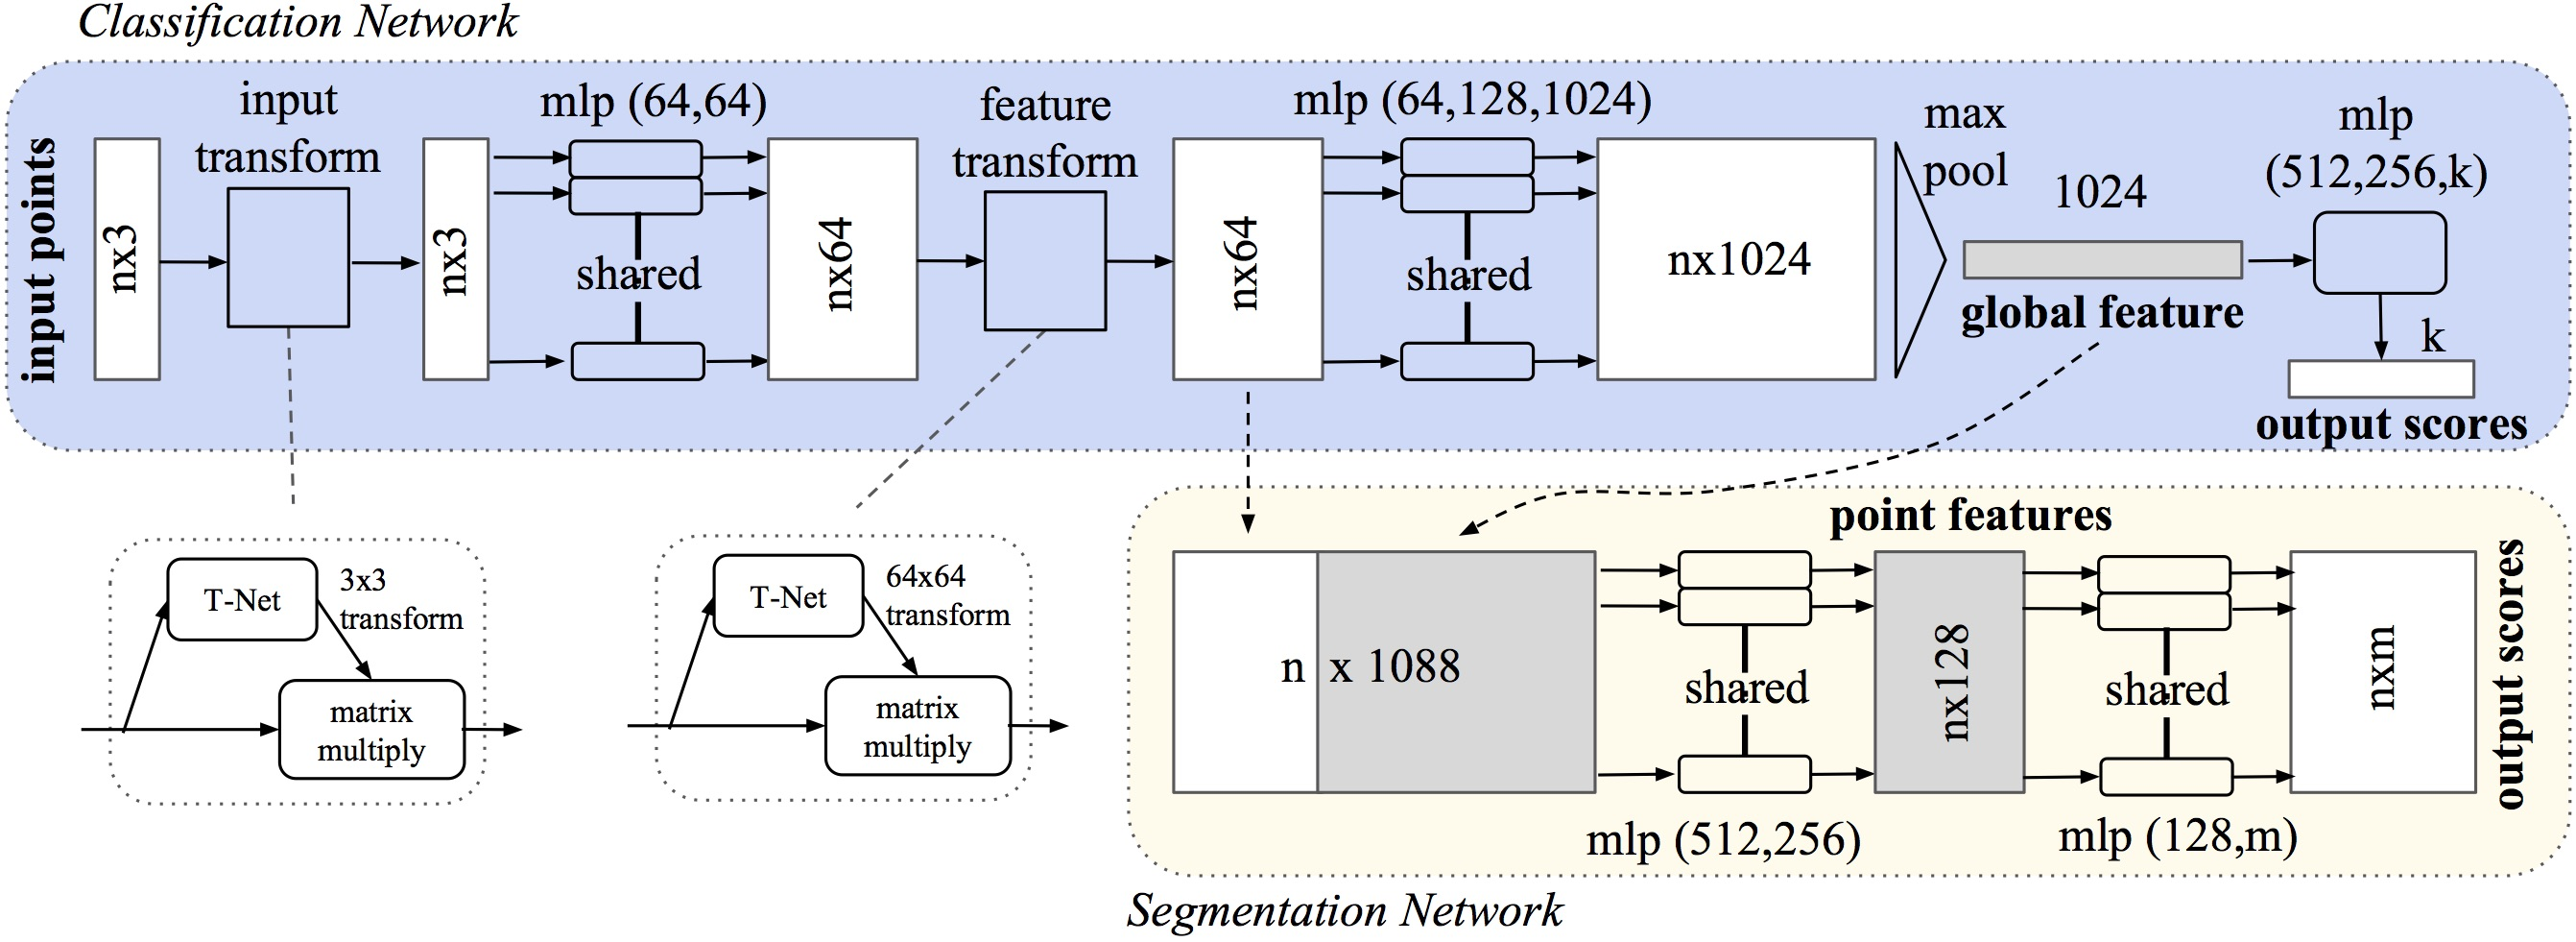
\includegraphics[scale=0.16]{Graphics/pointnet.jpg}
	\caption{PointNet architecture. Image from \cite{PointNet2017}.}
	\label{fig:pointnet}
\end{figure}

\section{Tools} % mention the edits on sponza and corridor and office, if any
In this section, technologies, tools, and assets used throughout this thesis will be briefly presented.

\subsection{Graphics Engine}
For the implementation of this thesis, a stable and well-documented engine with a variety of capabilities, especially supporting light probe features, was necessary. For that reason, we decided to use the Unity Engine. Unity is used globally for computer applications, ranging from 2D and 3D interactive applications like video games, simulations of physics interactions like liquid simulations, and cinematic films with realistic or stylized visuals. Unity additionally supports light probes internally, under the name Light Probe Groups, an object that contains all individual light probes of a scene and handles the interpolation and mapping of dynamic objects passing through the scene that are affected by GI.

\subsection{Sentis}
For the purposes of this thesis, a tool that allows us to run AI models inside Unity was needed. For that purpose, we used Sentis, a neural-network inference library for Unity. It is able to detect and import pre-trained AI models into Unity as assets, run them both in runtime and edit time, and utilize the end-user's device compute, CPU or GPU. Sentis is able to capture an .onnx file containing the AI model, and then exposes a variety of functions via programming code to allow the developer to send data to the model and capture the output of the model.

\subsection{3D Scenes}
For training and testing the AI model, we used the Sponza scene \parencite{Sponza2017}, the Office scene \parencite{Office2021}, and the Corridor scene \parencite{Corridor2021}. The scenes underwent some manual editing to make them better suit our needs, remove assets deemed unnecessary for our goals, or to import them properly inside Unity along with their textures and required objects. These edits are minimal and not vital to the thesis. Therefore, they will not be explicitly described.

\begin{figure}[h]
	\centering
	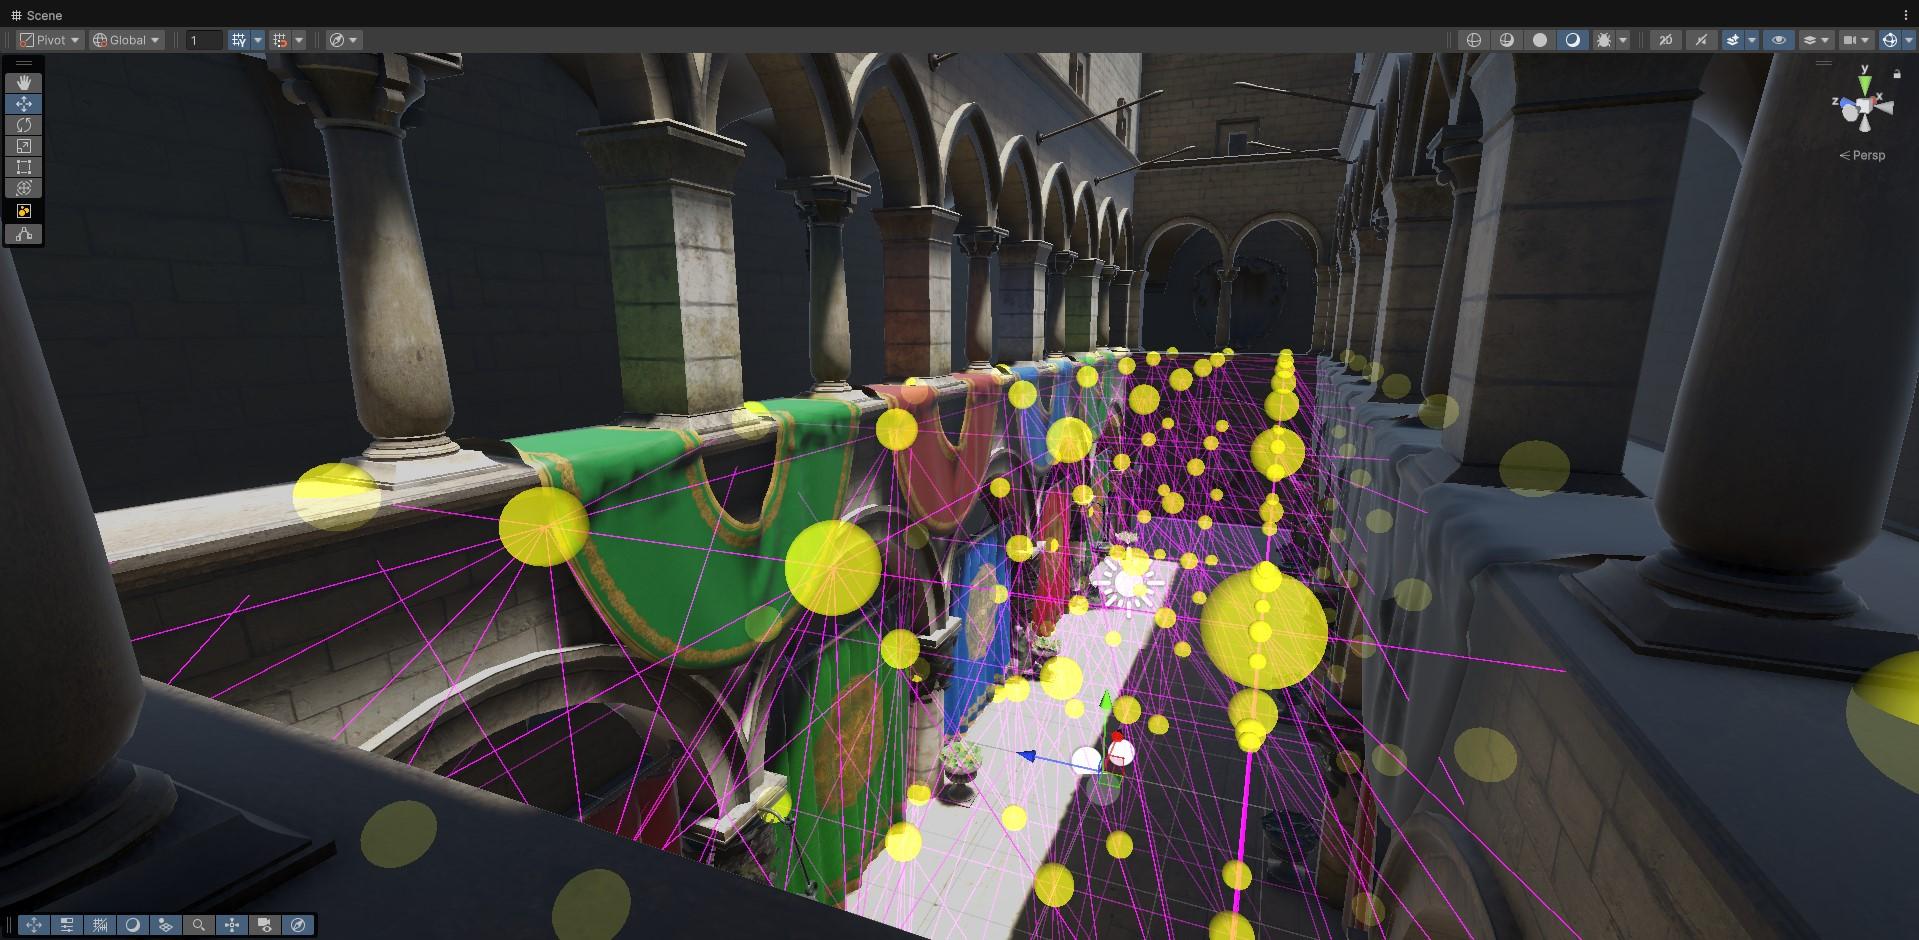
\includegraphics[scale=0.294]{Graphics/Sponza_lightprobes.jpg}
	\caption{The Sponza Unity Scene showing light probes placed on a grid \parencite{Sponza2017}.}
	\label{fig:Sponza_lp}
\end{figure}


\subsection{Python and TensorFlow}
For this thesis, Python was used as the language of choice for the creation of our Deep Learning AI Model. Python is an interpreted programming language. Its high-level nature makes it ideal for general purpose scenarios and easy to work with. Python was used for its simplicity, making the reading, preparation, post-processing, and saving of the data a fast process during the development of LPNN.

TensorFlow is a free and open-source software library used for machine-learning and artificial-intelligence applications. It supports a variety of well-known programming languages, but for this thesis we used the Python version for creating and training our model.

% somewhere, write how we identify important locations for light probes